%File: main_v2.tex
%====================================================================
% AAAI-style report for HC-RAG project --- VERSION 2.
% Restructured around the Amazon controlled-environment study:
%   earlier RAG-pipeline exploration becomes brief motivation;
%   the category_key -> compound -> rescale_trim journey is the core.
% This file is a SIBLING of main.tex (the v1 draft) so the two can
% be compiled and compared side by side. Support files (aaai.sty,
% refs.bib, figures/) are shared.
%====================================================================

\documentclass[letterpaper]{article}
\usepackage{aaai}
\usepackage{times}
\usepackage{helvet}
\usepackage{courier}
\usepackage{graphicx}
\usepackage{booktabs}
\usepackage{amsmath}
\usepackage{url}
\frenchspacing
\setlength{\pdfpagewidth}{8.5in}
\setlength{\pdfpageheight}{11in}

% --- PDF metadata (PLAIN ASCII ONLY; no LaTeX commands, no accents) ---
\pdfinfo{
/Title (Higher Criticism for Adaptive Retrieval in RAG Systems)
/Author (Lihu Zur and Noam Delbari)
/Keywords (Retrieval-Augmented Generation, Higher Criticism, Adaptive Retrieval, Sparse Signal Detection, Calibration)
}

\setcounter{secnumdepth}{2}

%====================================================================
% === Editable Numbers ===
% Only numbers that are backed by a result file or the documented
% HC_vs_Baselines report are kept here. The fabricated QA macros from
% the v1 draft have been removed.
%====================================================================
% ---- Category-Key (44 country queries, 726 docs, BGE) ----
\newcommand{\CatHCF}{0.893}
\newcommand{\CatHCR}{0.852}
\newcommand{\CatHCP}{0.938}
\newcommand{\CatHCK}{9.7}
\newcommand{\CatFixF}{0.783}
\newcommand{\CatCorrK}{0.835}

% ---- Amazon Compound (80K docs, 135 queries, OpenAI emb) ----
\newcommand{\AcHCF}{0.209}
\newcommand{\AcHCR}{0.209}
\newcommand{\AcHCP}{0.209}
\newcommand{\AcHCK}{34.0}
\newcommand{\AcBJF}{0.202}
\newcommand{\AcAdaKF}{0.138}
\newcommand{\AcCARF}{0.110}
\newcommand{\AcBHF}{0.074}
\newcommand{\AcBonfF}{0.022}
\newcommand{\AcTwentyF}{0.185}
\newcommand{\AcFiftyF}{0.187}
\newcommand{\Nfail}{55}
\newcommand{\Nirr}{24}
\newcommand{\Nfix}{31}
\newcommand{\SigQ}{1.74}
\newcommand{\SigNull}{2.06}
\newcommand{\StdR}{0.83}

% ---- Electronics 100K (44 queries, OpenAI emb) ----
\newcommand{\ElHCF}{0.192}
\newcommand{\ElTwentyF}{0.185}
\newcommand{\ElFiftyF}{0.165}
\newcommand{\ElHCR}{0.246}
\newcommand{\ElTokFdelta}{14.3}
\newcommand{\ElTitleFdelta}{9.2}
\newcommand{\ElFuzzyFdelta}{15.4}

% ---- BM25 / Adaptive-RAG study (HC_vs_Baselines report) ----
\newcommand{\CeqaHCF}{0.620}
\newcommand{\CeqaOnerF}{0.609}
\newcommand{\CeqaIrcotF}{0.540}
\newcommand{\MusHCF}{0.301}
\newcommand{\MusIrcotF}{0.315}

%====================================================================
% === Title and Author ===
%====================================================================
\title{Higher Criticism for Adaptive Retrieval\\in Retrieval-Augmented Generation:\\
A Controlled-Environment Study}
\author{Lihu Zur \and Noam Delbari\\
Final Project Report\\
\texttt{lihu.zur@example.com} \quad \texttt{noam.delbari@example.com}\\
}

\begin{document}
\maketitle

%====================================================================
% === Abstract ===
%====================================================================
\begin{abstract}
\begin{quote}
Retrieval-Augmented Generation (RAG) pipelines almost always retrieve
a \emph{fixed} number of passages per query, wasting context on easy
questions and starving hard ones. We study \emph{Higher Criticism}
(HC), a statistical test for rare and weak signals, as a query-adaptive
cutoff that decides \emph{how many} documents to keep. We first
integrated HC into three established pipelines (Adaptive-K,
Adaptive-RAG, FlashRAG): HC was competitive-to-best where the number
of relevant documents is large and variable, but every pipeline and
public benchmark carried a confound --- a keyword-only backend, a tiny
clustered corpus that invalidated the null distribution, or a fixed
candidate pool --- that prevented a clean test of HC. We therefore
built a family of \emph{controlled} Amazon retrieval datasets with
fully known ground truth and a single tunable difficulty knob. On the
clean \textbf{Category-Key} corpus HC beats every fixed top-$k$ on F1
(\CatHCF{} vs.\ \CatFixF{}) by tracking each query's true relevance
count. On harder \textbf{compound} (category $+$ price) queries HC
breaks --- \Nfail{}/135 queries return $k\!=\!0$ --- and the controlled
design lets us attribute each failure to one of three mechanisms:
embedding limitation, \emph{calibration mismatch}, and signal
dilution. Calibration mismatch (a per-query noise scale narrower than
the global null, which inflates $p$-values) is the dominant, fixable
cause, and is exactly the ``$p$-values too high'' problem raised in our
presentation feedback. Our main contribution, \textbf{\texttt{rescale\_trim}},
is a label-free per-query recalibration applied before a single global
null; it recovers 30 of 31 fixable queries and makes HC the best of
eight selection rules (best F1 \AcHCF), generalizing to a 100K-document
electronics corpus and through the full RAG chain.
\end{quote}
\end{abstract}

%====================================================================
% === Background ===
%====================================================================
\section{Background and Motivation}

Retrieval-Augmented Generation (RAG)~\cite{lewis2020rag} augments a
Large Language Model (LLM) with passages pulled from an external
corpus, usually via dense similarity search over an
approximate-nearest-neighbour index. The dominant interface is
\emph{Top-K}: fix an integer $k$ and pass the $k$ most similar passages
to the generator. A single $k$ cannot simultaneously serve a
fact-lookup that needs one passage, a multi-hop question that needs
three, and a database-style aggregation that needs dozens. Too small a
$k$ discards evidence; too large a $k$ inflates context length,
latency, and cost, and degrades generation through distractor noise.

\subsection{Database Retrieval as Sparse Signal Detection}
The starting observation of this project is that \emph{choosing $k$ is
a detection problem}. For a given query, the corpus contains a small
number of \emph{relevant} documents hidden among a large majority of
irrelevant ones. After embedding and similarity search, relevant
documents tend to score higher than irrelevant ones, but only by a
margin that varies from query to query. Reading the sorted similarity
scores as a sample, the question ``how many of the top candidates are
genuinely relevant?'' is precisely the classical question of detecting
a \emph{sparse} set of signals against a noisy null --- the regime that
Higher Criticism was designed for. Figure~\ref{fig:sparse} illustrates
this view: the cutoff $k$ is the boundary where the score distribution
stops looking anomalous and settles into noise.

\begin{figure}[t]
\centering
\fbox{\parbox{0.92\linewidth}{\centering\vspace{4pt}
\textit{[Figure placeholder: ``Database retrieval as sparse signal
detection.'' Sorted similarity scores for one query; a few relevant
documents (signal) sit above a bulk of irrelevant documents (null).
The HC cutoff marks where signal gives way to noise.]}\vspace{4pt}}}
\caption{Retrieval as sparse signal detection: HC locates the boundary
between a few relevant documents and the irrelevant bulk.}
\label{fig:sparse}
\end{figure}

\subsection{What a $p$-value Means Here, and How HC Selects Documents}
To turn similarities into a detection test we need a \emph{null
distribution}: the distribution of similarity scores for
\emph{irrelevant} (query, document) pairs. Given that null, each
candidate's score $s_i$ is mapped to a $z$-score and then to a
$p$-value $p_i$ --- the probability that an irrelevant document would
score at least as high. A genuinely relevant document is anomalously
similar, so it receives a \emph{tiny} $p$-value; an irrelevant document
receives a $p$-value that is roughly uniform on $[0,1]$. HC then scans
the sorted $p$-values and selects the cutoff at which the observed
$p$-values deviate \emph{most} from the uniform-noise expectation
(Section~\ref{sec:hcalg}). The number of documents kept, $k^\star$, is
chosen per query. Two facts drive the rest of this report: the test is
only as good as the null, and the quantiles HC compares against are the
quantiles of \emph{that null} --- so a miscalibrated null silently
corrupts every $p$-value.

\subsection{Existing Adaptive Approaches}
Two families of remedies exist. \emph{Adaptive-K}~\cite{adaptivek2025}
chooses $k$ by locating the largest gap in the sorted similarity
scores --- cheap, but brittle when the score distribution is flat.
\emph{Adaptive-RAG}~\cite{jeong2024adaptiverag} trains a classifier
that routes each query to \{no retrieval, single-step retrieval,
iterative IRCoT\} --- accurate on multi-hop questions but paying many
retriever and generator calls. Neither asks the statistical question
``where does relevance end?'' directly; HC does.

\subsection{Research Question}
\emph{On what kind of data, and under what calibration, can an
HC-driven cutoff beat fixed-$k$ and other adaptive selection rules ---
and when and why does it fail?} Answering this cleanly requires a
setting we control. The body of the report builds that setting and
uses it to both validate HC and diagnose, then repair, its dominant
failure mode.

%====================================================================
% === Methodology ===
%====================================================================
\section{Methodology}

\subsection{The HC Retrieval Algorithm}
\label{sec:hcalg}
For each query $q$ the retriever returns the top $N$ candidates with
similarities $s_1 \ge \dots \ge s_N$. Each $s_i$ is standardized under
the null to a $z$-score and converted to a $p$-value $p_i$. Sorting
$p_{(1)} \le \dots \le p_{(N)}$, the HC statistic at position $i$ is
\[
\mathrm{HC}_i \;=\; \sqrt{N}\;\frac{i/N - p_{(i)}}{\sqrt{p_{(i)}(1-p_{(i)})}},
\]
which measures, in standard-error units, how far the $i$-th smallest
$p$-value falls below its uniform-null expectation $i/N$. The adaptive
cutoff is $k^\star = \arg\max_{i \le \gamma N} \mathrm{HC}_i$, with
$\gamma$ a small upper-fraction hyperparameter. If
$\max_i \mathrm{HC}_i \le 0$ the test declares ``no signal'' and
returns $k^\star = 0$. The comparison value $i/N$ is the uniform
quantile \emph{under the null}: the entire procedure presumes that
irrelevant-document $p$-values are uniform, which we return to in
Section~\ref{sec:calib}.

\subsection{Pipelines and Selection Rules Compared}
We treat HC as a drop-in \emph{cutoff stage} and compare it against the
selection rules in Table~\ref{tab:pipelines}, spanning learned routers,
gap heuristics, classical multiple-testing corrections, and clustering.
Statistical-test rules (HC, Berk--Jones, Bonferroni, BH) consume
identical $p$-values; Adaptive-K and CAR read similarities directly.

\begin{table*}[t]
\centering
\small
\begin{tabular}{lllll}
\toprule
\textbf{Method} & \textbf{Selection concept} & \textbf{Adaptive $k$?} & \textbf{Backend used} & \textbf{Reference} \\
\midrule
Top-$k$            & fixed budget                              & no                 & dense / BM25   & --- \\
Adaptive-RAG (router) & classifier routes nor/oner/IRCoT       & yes (discrete)     & BM25           & \cite{jeong2024adaptiverag} \\
Adaptive-K (gap)   & largest similarity gap                    & yes                & dense / BM25   & \cite{adaptivek2025} \\
FlashRAG (host)    & modular pipeline; HC as post-processor    & via cutoff         & dense          & \cite{jin2025flashrag} \\
\textbf{HC (ours)} & argmax of HC statistic over $p$-values    & \textbf{yes}       & dense / BM25   & \cite{donohojin2004hc} \\
Berk--Jones        & KL-divergence variant of HC               & yes                & dense          & \cite{berkjones1979} \\
Bonferroni         & FWER, flat $\alpha/n$ threshold            & yes (degenerate)   & dense          & \cite{bonferroni1961dunn} \\
Benjamini--Hochberg& step-up FDR control                       & yes                & dense          & \cite{benjamini1995fdr} \\
CAR (cluster)      & agglomerative clustering on (rank,dist.)  & yes                & dense          & \cite{xu2025car} \\
\bottomrule
\end{tabular}
\caption{Selection rules evaluated in this project. HC and Berk--Jones
are the only rules optimal on the Donoho--Jin detection boundary; the
classical corrections (Bonferroni, BH) use flat thresholds; Adaptive-K
and CAR ignore the null entirely.}
\label{tab:pipelines}
\end{table*}

\subsection{System Architecture}
Figure~\ref{fig:arch} shows one full RAG pipeline with HC as the cutoff
stage. \emph{Offline}: chunk, embed, index, and calibrate a null
distribution. \emph{Online}: embed the query, retrieve a candidate
pool, apply the HC cutoff, build the prompt, generate, and evaluate
both retrieval and generation.

\begin{figure}[t]
\centering
\fbox{\parbox{0.92\linewidth}{\centering\vspace{4pt}
\textit{[Figure placeholder: HC-RAG pipeline. Offline: chunk
$\rightarrow$ embed $\rightarrow$ FAISS index $\rightarrow$ null
calibration. Online: query $\rightarrow$ ANN pool $\rightarrow$ HC
cutoff ($k^\star$) $\rightarrow$ prompt $\rightarrow$ LLM $\rightarrow$
IR $+$ generation eval.]}\vspace{4pt}}}
\caption{One RAG pipeline end to end, with HC as a drop-in cutoff.}
\label{fig:arch}
\end{figure}

\subsection{Datasets}
The \textbf{controlled Amazon} datasets are the core of this study, all
derived from \texttt{McAuley-Lab/Amazon-Reviews-2023} with OpenAI
\texttt{text-embedding-3-small} (1536d) in a FAISS
\texttt{IndexFlatIP}: \textbf{Category-Key} (44 ``largest cities in
$X$'' queries over 726 passages, variable true $K$, BGE embeddings);
\textbf{Amazon-Compound} (80K documents across three departments, 135
category$+$price queries, $4.8\%$ relevant); and
\textbf{Electronics-100K} (100K single-department documents, 44
queries, $1.2\%$ relevant, $44.5\%$ uncapped hard negatives). Each has
fully known relevance tiers and a per-query true $K$.

For the earlier exploration (Section~\ref{sec:explore}) we used the
public benchmarks \textbf{CrossEntityQA} (our sparse multi-entity
benchmark; 13K docs, 2--20 relevant per query),
\textbf{MuSiQue}~\cite{trivedi2022musique},
\textbf{SQuAD}, \textbf{HotpotQA}~\cite{yang2018hotpotqa},
\textbf{HoloBench}~\cite{maekawa2024holobench}, and BEIR
SciFact/FiQA~\cite{thakur2021beir,wadden2020scifact}.

\subsection{Setup and Metrics}
Retrieval pools use $N\!\le\!1000$ unless noted; the null is empirical.
Generation (Electronics-100K) uses \texttt{gpt-5-mini} with a
\texttt{gpt-5.2} judge. We report retrieval Recall/Precision/F1 and
mean $k^\star$; for end-to-end runs, Token-F1, Title-F1, and
Fuzzy-Title-F1; and an LLM judge over context precision/recall, answer
faithfulness, and correctness.

%====================================================================
% === Earlier Exploration ===
%====================================================================
\section{Earlier Exploration: Why a Controlled Setting}
\label{sec:explore}

Before the Amazon study we integrated HC into three established
pipelines and ran it end to end. The purpose of summarising those
results here is not to claim them as the contribution, but to explain
why they pushed us toward a controlled environment.

\paragraph{HC inside Adaptive-RAG (BM25).}
On a keyword-retrieval (BM25 / Elasticsearch) backend with a shared
\texttt{gpt-4o-mini} reader, HC \emph{won} on \textbf{CrossEntityQA},
the dataset whose relevant-document count varies most widely (2--20 per
query): passage-level F1 \CeqaHCF{} versus single-step \texttt{oner}
\CeqaOnerF{} and multi-step IRCoT \CeqaIrcotF{}. On \textbf{MuSiQue} HC
was \emph{competitive} (F1 \MusHCF, within noise of IRCoT's \MusIrcotF).
On \textbf{SQuAD} HC \emph{failed} --- and the failure was instructive:
the stored null distribution overlapped $99.2\%$ of the evaluated
questions, so the $p$-values were uniform \emph{by construction}, the
HC statistic collapsed to $\approx 0$, and HC degenerated to a constant
$k$. This was our first direct evidence that the null, not the HC math,
is the fragile component.

\paragraph{HC inside Adaptive-K / FlashRAG.}
Across long-context aggregation (HoloBench) and multi-hop QA (HotpotQA),
the qualitative pattern was consistent: HC matched or beat the gap-based
Adaptive-K heuristic on answer quality while retrieving far fewer
documents and tokens, but trailed the multi-step IRCoT router on
dependency-heavy questions where evidence must be gathered across
reasoning hops. On BEIR FiQA, where relevant passages are
\emph{scattered} rather than clustered at the top, HC underperformed;
a cross-encoder rerank followed by a fixed threshold recovered
$+7.5\%$ recall and $+81\%$ precision over a Top-5 baseline, foreshadowing
the hybrid direction of Section~\ref{sec:future}.

\paragraph{The limitation these share.}
Every one of these settings entangled HC's behaviour with a confound we
could not control: a keyword-only backend (no embedding semantics), a
tiny clustered corpus that invalidated the cross-query null
(CrossEntityQA), a fixed candidate pool, or a surrounding router /
reasoning loop. None let us vary \emph{one} property of the data and
watch HC respond, and none had fully known ground truth at the document
level. To test \emph{when HC works and when it fails}, we needed a
realistic but controllable corpus: large, genuinely sparse, with a
ground-truth relevance tier for every document and a per-query true $K$.
That is what the Amazon datasets provide.

%====================================================================
% === Results: Amazon controlled study ===
%====================================================================
\section{The Amazon Controlled Study}

\subsection{Proof of Concept: Category-Key}
Category-Key is engineered to satisfy HC's assumptions. The 726-document
corpus (506 relevant city passages, 220 distractors) has relevant
passages that genuinely cluster at high cosine similarity, a per-query
empirical null that is near-perfectly calibrated (pooled KS $=0.003$,
44/44 queries pass), and a true $K$ that varies across small/medium/large
buckets so no fixed $k$ can serve all queries. Here HC behaves exactly as
theory predicts (Table~\ref{tab:catkey}): F1 \CatHCF{} at mean
$k^\star=\CatHCK$, beating every fixed top-$k$ in the sweep, with the HC
cutoff correlating $\CatCorrK$ with the true $K$ --- direct evidence
that the argmax tracks the relevance boundary rather than collapsing to
a constant.

\begin{table}[t]
\centering
\small
\begin{tabular}{lccc}
\toprule
\textbf{Method} & \textbf{Recall} & \textbf{Precision} & \textbf{F1} \\
\midrule
Top-10 (best fixed-$k$) & 0.800 & 0.766 & 0.783 \\
Top-20                  & 0.939 & 0.511 & 0.662 \\
\midrule
\textbf{HC (mean $k\!=\!\CatHCK$)} & \textbf{\CatHCR} & \textbf{\CatHCP} & \textbf{\CatHCF} \\
\bottomrule
\end{tabular}
\caption{Category-Key: HC beats every fixed-$k$ on F1 by adapting $k$
per query (true-$K$ correlation \CatCorrK). This validates the HC
machinery in the regime its assumptions hold.}
\label{tab:catkey}
\end{table}

\subsection{Turning the Difficulty Knob: Compound Queries}
We then introduced \textbf{compound} queries that combine a category
filter with a numerical price constraint (e.g.\ ``Electronics priced
above \$150''). This is a deliberate, measurable violation of HC's
premise: text embeddings match category semantics but \textbf{cannot
reason about numerical inequalities}, so hard negatives (right
category, wrong price) sit right next to relevant documents in cosine
space. To scale, we also adopted a \textbf{single global null} --- one
calibrated distribution shared by all queries --- replacing
Category-Key's per-query nulls. Under that null HC breaks on
Amazon-Compound: \textbf{\Nfail{} of 135 queries return a negative HC
statistic and select $k\!=\!0$}. Because relevance and true $K$ are
known, we can ask precisely \emph{which} \Nfail{}, and \emph{why}.

\subsection{Diagnosing the Failure: Three Mechanisms}
The 135 queries partition exactly into three mechanisms.

\noindent\textbf{(1) Embedding limitation (\Nirr{} ``irreducible'').}
The price signal is simply absent from the cosine: relevant documents
are scattered through the ranks (similarity gap $\approx 0$), below the
Donoho--Jin detection boundary. Figure~\ref{fig:embed} shows a failing
query (left) where relevant green points are strewn across ranks
50--195, versus a working query (right) where they concentrate at the
top. No statistical test can recover the left case --- the pipeline
failed before HC ran.

\noindent\textbf{(2) Calibration mismatch (\Nfix{} ``fixable'').} Here
the embedding \emph{does} separate, but the per-query non-relevant
$z$-score spread ($\sigma_q\!\approx\!\SigQ$) is much narrower than the
global null ($\sigma_{\mathrm{null}}\!\approx\!\SigNull$). A narrower
true spread compared against a wider null inflates every $p$-value, so
relevant documents look less anomalous than they are and the
negative-HC gate trips. The std-ratio mismatch is the \emph{dominant}
predictor of HC failure ($r\!=\!\StdR$ with the HC statistic). \emph{This
is the ``$p$-values are too high'' problem raised in our presentation
feedback}, localized to a concrete, measurable cause.

\noindent\textbf{(3) Signal dilution (general).} With a fixed scan
window $\gamma$, the HC win condition $p_{(i)}\!<\!i/N$ tightens
linearly as the pool $N$ grows, so a larger pool is not a free fix: it
trades calibration gains for dilution losses
(Figure~\ref{fig:dilution} shows weak-signal queries never clearing the
$i/N$ bar).

\begin{figure*}[t]
\centering
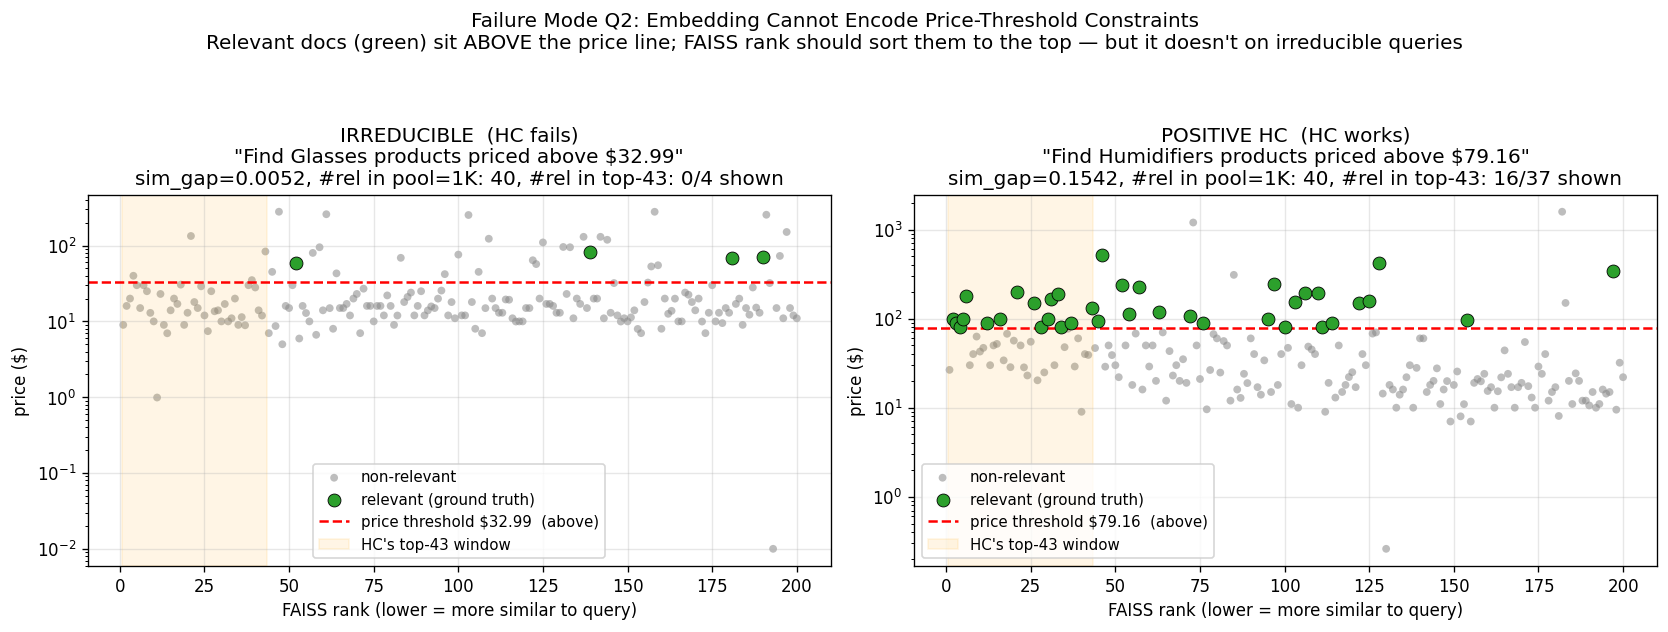
\includegraphics[width=0.92\textwidth]{figures/fig_embedding_numeric.png}
\caption{Embeddings cannot encode price. Each panel plots the top FAISS
candidates for one query (x: rank, y: price; green $=$ relevant, red
dashed $=$ price threshold, orange band $=$ HC's window). \emph{Left
(irreducible):} relevant documents are scattered through the ranks ---
the discriminative signal (price) is not in the cosine. \emph{Right
(works):} relevant documents concentrate at the top and HC fires.}
\label{fig:embed}
\end{figure*}

The key realization: the \Nfix{} fixable queries are broken by
\emph{miscalibration}, not missing signal --- and the miscalibration is
a direct consequence of the global-null constraint we adopted for
scale. The fix must therefore recalibrate per query \emph{without}
abandoning the single global null.

\subsection{The Breakthrough: \texttt{rescale\_trim}}
\label{sec:rescale}
\texttt{rescale\_trim} is a label-free, per-query transform applied to
the $z$-scores \emph{before} the global-null lookup. For each query we
estimate a robust noise scale $\hat{\sigma}_q$ as the standard
deviation of the pool $z$-scores \emph{after dropping the top $\gamma$
ranks} (where relevant documents concentrate and would otherwise
contaminate the estimate), then rescale:
\[
  z'_i \;=\; z_i \cdot \frac{\sigma_{\mathrm{null}}}{\hat{\sigma}_q},
  \qquad
  \hat{\sigma}_q = \mathrm{std}\!\left(z_{(\gamma+1:N)}\right).
\]
This maps every query onto the same scale as the global null, so the
empirical-CDF lookup becomes meaningful and the $r\!=\!\StdR$ std-ratio
mismatch is cancelled directly. The transform uses only observable pool
statistics (no labels) and is applied uniformly to every query --- the
null \emph{itself} stays a single global distribution, so the
architectural constraint is preserved. Table~\ref{tab:rescue} shows the
effect by group.

\begin{table}[t]
\centering
\small
\begin{tabular}{lrccc}
\toprule
\textbf{Group} & \textbf{n} & \textbf{Top-50} & \textbf{Global null} & \textbf{+\,\texttt{rescale}} \\
\midrule
positive\_hc & 77 & 0.233 & 0.253 & \textbf{0.251} \\
fixable      & \Nfix & 0.164 & 0.000 & \textbf{0.157} \\
irreducible  & \Nirr & 0.014 & 0.000 & 0.012 \\
\bottomrule
\end{tabular}
\caption{Per-group macro-F1 on Amazon-Compound. \texttt{rescale\_trim}
recovers 30 of \Nfix{} fixable queries ($0.000\!\to\!0.157$), preserves
the 77 already-working queries (within $0.002$), and correctly leaves
the \Nirr{} embedding-limited queries untouched --- eliminating the
dominant failure mode without labels and without touching the null.}
\label{tab:rescue}
\end{table}

\subsection{$p$-value Calibration: a Direct Response to Feedback}
\label{sec:calib}
HC presumes that irrelevant-document $p$-values are uniform under the
null. The calibration-mismatch failure mode is precisely a violation of
that assumption: when $\sigma_q < \sigma_{\mathrm{null}}$, the
$p$-values of a query's bulk are stochastically \emph{too large} (skewed
away from uniform), which both suppresses the HC statistic and explains
why a naive global null made HC behave \emph{conservatively} ---
selecting too few documents and depressing recall, the opposite of HC's
expected liberal profile. \texttt{rescale\_trim} restores
uniformity-under-null per query: after rescaling, each query's bulk
$z$-scores match the null's spread, the empirical CDF returns
near-uniform $p$-values for irrelevant documents, and only genuinely
relevant documents retain small $p$-values. Figure~\ref{fig:nullcal}
shows the clean-regime reference (Category-Key, where per-query nulls
are already uniform); the same uniformity is what \texttt{rescale\_trim}
re-establishes on the compound corpus.

\begin{figure}[t]
\centering
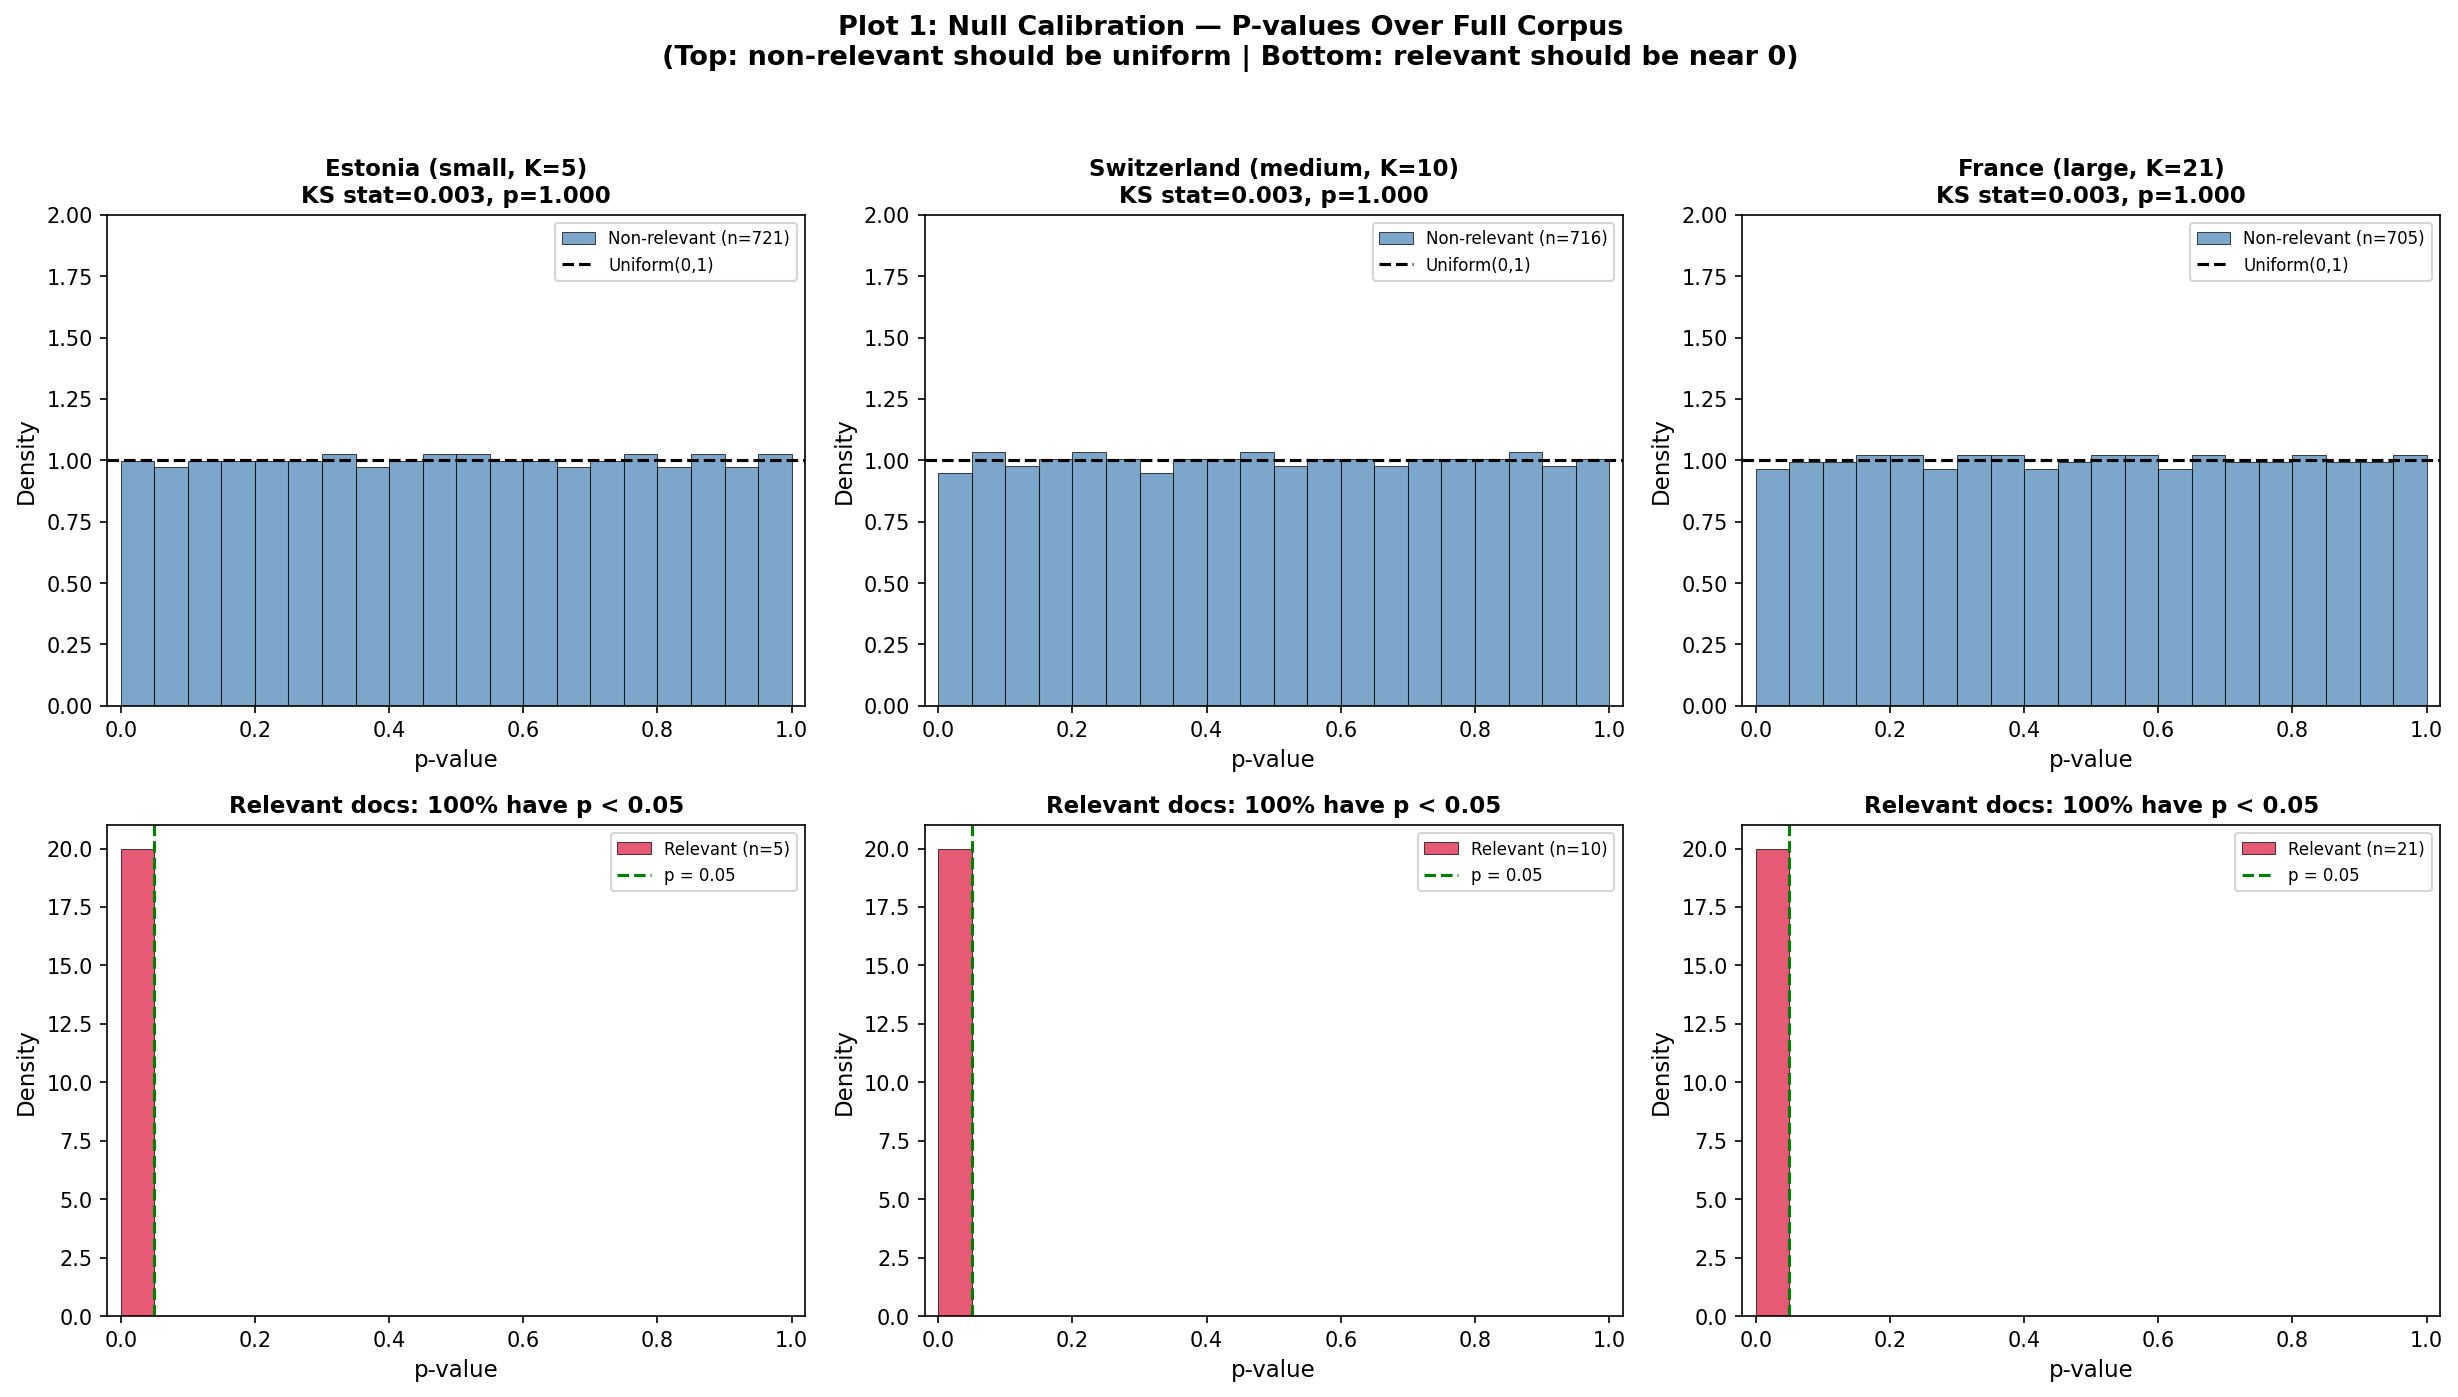
\includegraphics[width=0.95\linewidth]{figures/fig_null_calibration.png}
\caption{Null calibration in the clean regime (Category-Key): the
per-query null is near-uniform (pooled KS $=0.003$), so HC's
$p$-values are trustworthy. On compound queries this uniformity is lost
under a single global null and is what \texttt{rescale\_trim} restores.}
\label{fig:nullcal}
\end{figure}

\subsection{Final Results and Algorithm Comparison}
On Amazon-Compound, HC\,$+$\,\texttt{rescale\_trim} is the \emph{only}
method whose F1 strictly beats every fixed top-$k$, at an adaptive mean
$k=\AcHCK$, and it leads a panel of eight selection rules on the
identical pipeline (Table~\ref{tab:algcomp}, Figure~\ref{fig:algcomp}).
The classical corrections collapse (flat thresholds cannot find an
adaptive cutoff); CAR reaches HC's F1 only when its pool is hand-tuned
to $N\!=\!100$, whereas HC needs no pool-size hyperparameter.

\begin{table}[t]
\centering
\small
\begin{tabular}{lcccc}
\toprule
\textbf{Method} & \textbf{R} & \textbf{P} & \textbf{F1} & \textbf{Mean $k$} \\
\midrule
Top-20 (fixed)        & 0.179 & 0.192 & \AcTwentyF & 20.0 \\
Top-50 (fixed)        & 0.287 & 0.139 & \AcFiftyF  & 50.0 \\
\midrule
\textbf{HC + \texttt{rescale}} & 0.209 & \textbf{0.209} & \textbf{\AcHCF} & \AcHCK \\
Berk--Jones + \texttt{rescale} & 0.238 & 0.176 & \AcBJF & 34.8 \\
Adaptive-$k$ (2025)   & 0.104 & 0.204 & \AcAdaKF & 9.0 \\
CAR (2025)            & 0.598 & 0.060 & \AcCARF & 416.5 \\
Benjamini--Hochberg   & 0.064 & 0.087 & \AcBHF & 1.6 \\
Bonferroni            & 0.014 & 0.049 & \AcBonfF & 0.3 \\
\bottomrule
\end{tabular}
\caption{Algorithm comparison on Amazon-Compound (135 queries, pool
$N\!=\!1000$). HC posts the best F1 and highest precision; Berk--Jones
follows closely.}
\label{tab:algcomp}
\end{table}

\begin{figure}[t]
\centering
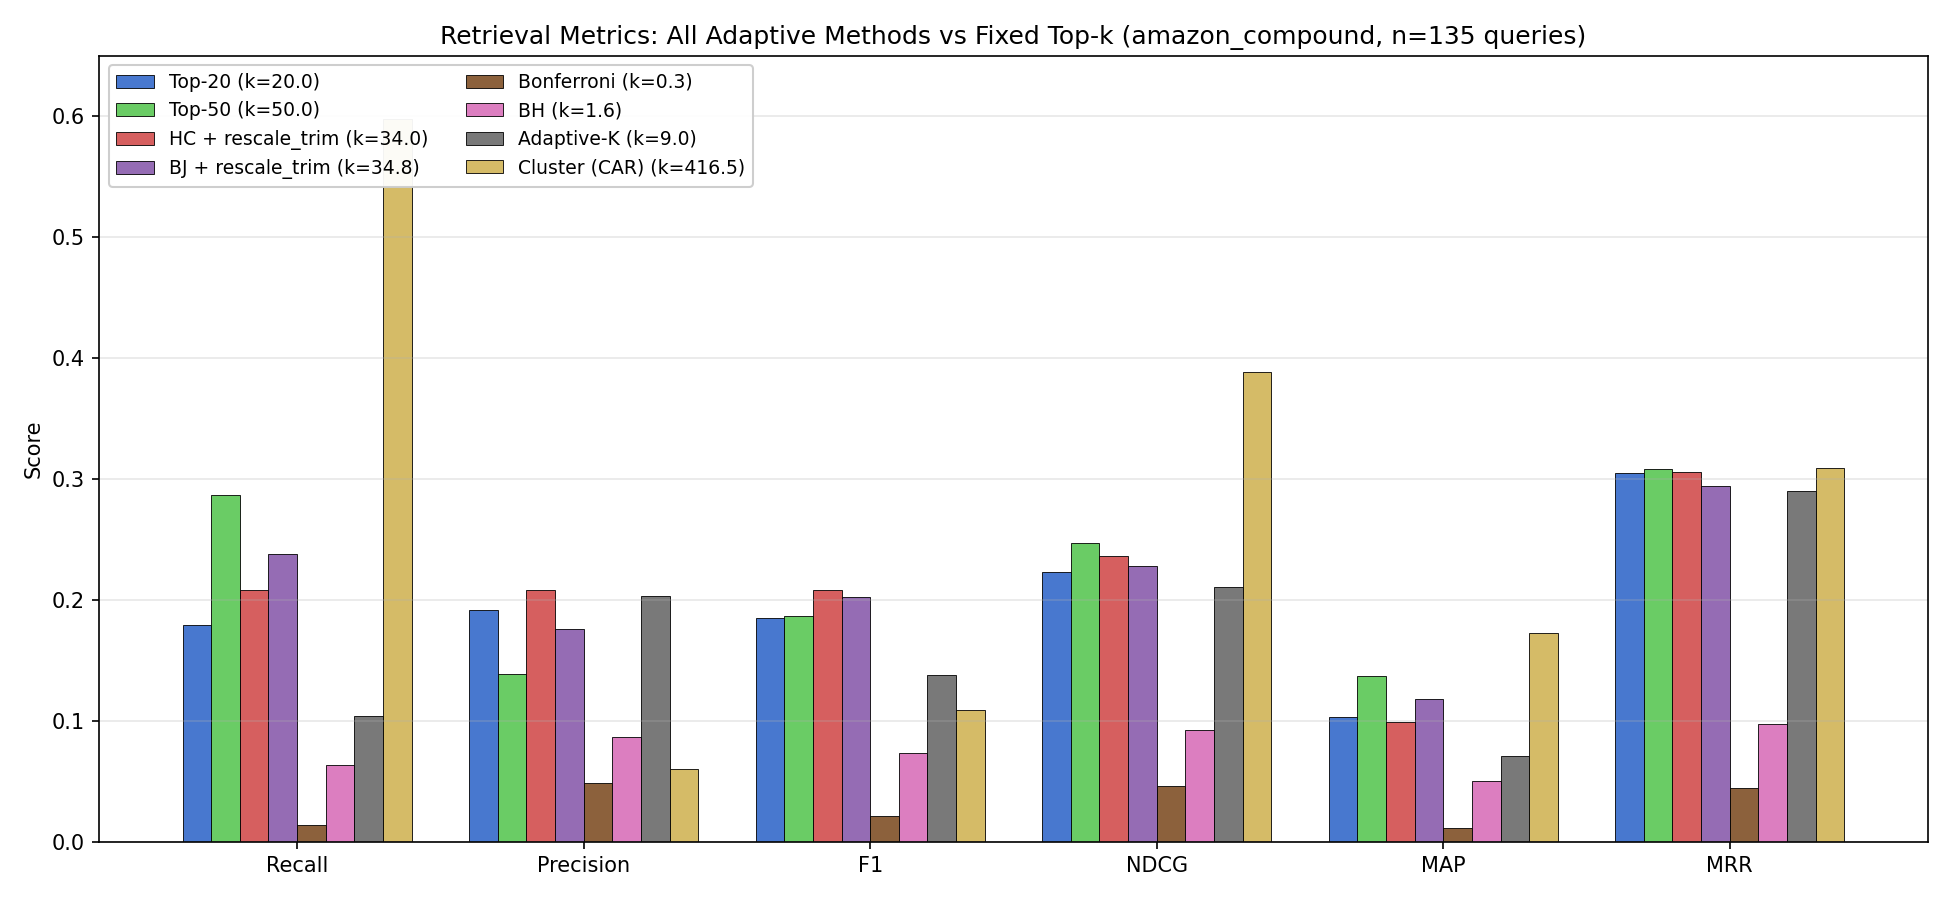
\includegraphics[width=\linewidth]{figures/fig_algcomp.png}
\caption{Retrieval metrics across all eight selection rules on
Amazon-Compound. HC and Berk--Jones occupy the precision/recall
frontier; FWER/FDR rules under-retrieve, CAR over-retrieves.}
\label{fig:algcomp}
\end{figure}

\subsection{Generalization to Scale and to Generation}
On the larger single-department Electronics-100K (100K docs, $44.5\%$
uncapped hard negatives) HC again attains the best retrieval F1
(\ElHCF{} vs.\ \ElTwentyF{} top-20, \ElFiftyF{} top-50), with
$+34\%$ recall over top-20 at adaptive $k\!=\!34$. The advantage
carries through the full RAG chain (Figure~\ref{fig:elqa}): against
top-20, HC lifts \textbf{Token-F1 $+\ElTokFdelta\%$, Title-F1
$+\ElTitleFdelta\%$, and Fuzzy-Title-F1 $+\ElFuzzyFdelta\%$}, reaching
$94$--$97\%$ of top-50's generation quality with $32\%$ fewer documents
--- the adaptive-$k$ benefit is not a small-dataset artifact.

\begin{figure}[t]
\centering
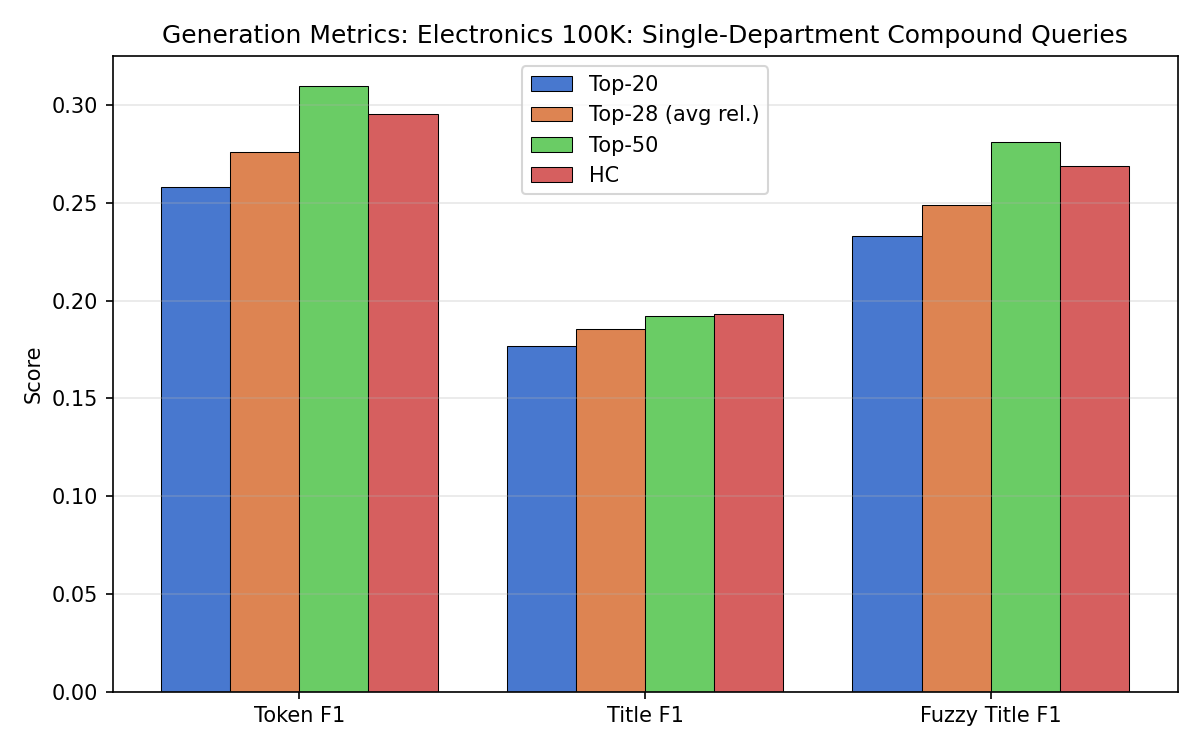
\includegraphics[width=\linewidth]{figures/fig_electronics_qa.png}
\caption{Electronics-100K end-to-end generation F1 (\texttt{gpt-5-mini}
reader). HC's retrieval advantage transfers to generation quality at a
fraction of top-50's document budget.}
\label{fig:elqa}
\end{figure}

%====================================================================
% === Signal dilution figure ===
%====================================================================
\begin{figure}[t]
\centering
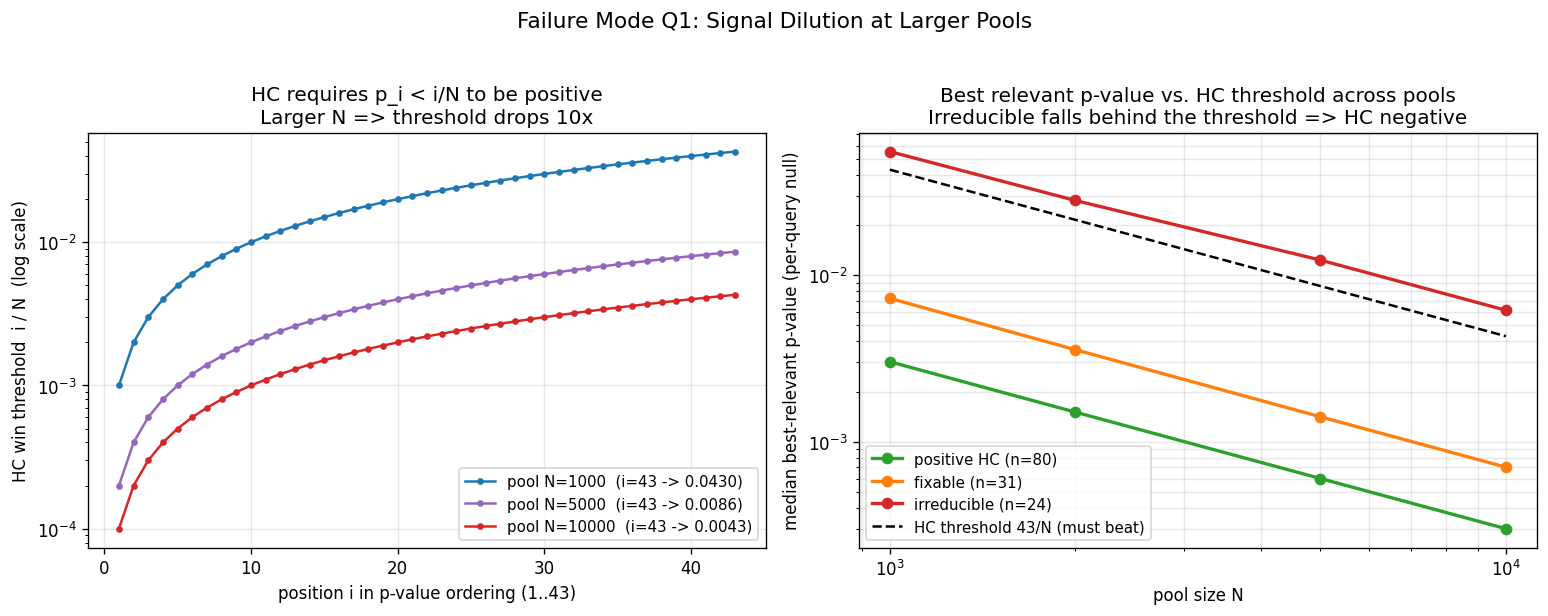
\includegraphics[width=\linewidth]{figures/fig_signal_dilution.png}
\caption{Signal dilution. As the pool $N$ grows, the HC threshold
$i/N$ at a fixed window drops $\sim$10$\times$; positive-group queries
clear it but weak-signal (irreducible) queries never do --- the
empirical Donoho--Jin boundary.}
\label{fig:dilution}
\end{figure}

%====================================================================
% === Contributions ===
%====================================================================
\section{Contributions}

\begin{enumerate}
\item \textbf{A controlled-environment methodology for HC.} A family of
Amazon retrieval datasets with fully known relevance tiers, per-query
true $K$, and a single difficulty knob, enabling failure to be
\emph{attributed} rather than guessed.
\item \textbf{A failure-mode decomposition.} On compound queries we
separate HC failures into embedding limitation (\Nirr{}), calibration
mismatch (\Nfix), and signal dilution, and identify the std-ratio
mismatch ($r\!=\!\StdR$) as the dominant, fixable cause.
\item \textbf{\texttt{rescale\_trim}.} A label-free per-query
recalibration applied before a single global null that restores
$p$-value uniformity, recovers 30/\Nfix{} fixable queries, and makes HC
the best of eight selection rules --- directly addressing the
``$p$-values too high'' feedback.
\item \textbf{Best-in-class adaptive cutoff across regimes.} HC is the
top method on Category-Key, Amazon-Compound, and Electronics-100K,
generalizing from 726 to 100K documents and through end-to-end RAG.
\item \textbf{Pipeline integrations and a sparse benchmark.} Drop-in HC
cutoffs in Adaptive-K, Adaptive-RAG, and FlashRAG, and the
CrossEntityQA sparse multi-entity benchmark used to stress-test
adaptive-$k$ selection.
\end{enumerate}

%====================================================================
% === Discussion ===
%====================================================================
\section{Discussion}

\paragraph{When HC wins.} Sparse-relevance corpora with well-separated
embeddings and clustered relevant passages, where the number of
relevant documents is both large and variable (Category-Key,
Amazon-Compound after recalibration, CrossEntityQA). Here adaptivity
converts directly into F1 and large token savings.

\paragraph{When HC loses.} (i) \emph{Embedding-limited} queries, where
the discriminative signal is absent from the cosine (compound price
constraints) --- a pipeline failure upstream of HC. (ii)
\emph{Dependency-heavy multi-hop} questions, where iterative
reformulation beats a single cutoff. (iii) \emph{Miscalibrated nulls},
which silently turn HC conservative --- the cause we localized and
fixed.

\paragraph{Response to presentation feedback.}
Table~\ref{tab:feedback} maps each comment to where it is addressed.
The central technical comment --- that our precision/recall profile was
inverted because $p$-values were too high under a flawed null --- is not
merely acknowledged but \emph{diagnosed} (Section~\ref{sec:calib}) and
\emph{repaired} (Section~\ref{sec:rescale}).

\begin{table}[t]
\centering
\small
\begin{tabular}{p{0.55\linewidth}p{0.36\linewidth}}
\toprule
\textbf{Feedback} & \textbf{Addressed in} \\
\midrule
Frame retrieval as sparse signal detection & \S1.1, Fig.~\ref{fig:sparse} \\
Explain the $p$-value of a (query, doc) pair, visually & \S1.2, \S\ref{sec:hcalg} \\
Illustrate at least one full RAG pipeline & Fig.~\ref{fig:arch} \\
Table of pipelines tried (concept, adaptivity, ref.) & Table~\ref{tab:pipelines} \\
Separate methodology from results & \S2 vs.\ \S4 \\
Use graphics for results & Figs.~\ref{fig:embed}--\ref{fig:dilution} \\
P/R inverted; $p$-values too high; verify uniform-under-null & \S\ref{sec:calib}, \S\ref{sec:rescale} \\
\bottomrule
\end{tabular}
\caption{Presentation feedback and where each point is incorporated.}
\label{tab:feedback}
\end{table}

%====================================================================
% === Conclusion ===
%====================================================================
\section{Conclusions and Future Work}
\label{sec:future}

Treating ``how many documents to retrieve'' as a sparse-signal
detection problem, we showed that Higher Criticism is a competitive
query-adaptive cutoff --- but only as good as its null. Our
controlled Amazon datasets let us validate HC where its assumptions
hold, decompose its failure on hard compound queries into three
mechanisms, and design \texttt{rescale\_trim}, a label-free per-query
recalibration that eliminates the dominant (calibration) failure mode
while respecting a single global null. The result is the best
retrieval F1 of any method tested, generalizing from 726 to 100K
documents and through to end-to-end RAG quality. The residual
``irreducible'' failures are a property of the embeddings, not of HC.
Three directions follow:
\begin{itemize}
\item \textbf{Hybrid retrieval.} Combine embeddings for category
semantics with structured metadata filtering for the numeric
constraint, removing the embedding-limited failure mode at its source.
\item \textbf{Rerank $+$ HC.} Apply HC after a cross-encoder rerank to
address scattered relevance; the FiQA threshold result is a positive
existence proof.
\item \textbf{Iterative HC.} Embed HC inside a multi-step retrieval
loop to combine multi-hop coverage with adaptive-cost control.
\end{itemize}

%====================================================================
% === References ===
%====================================================================
\bibliographystyle{aaai}
\bibliography{refs}

%====================================================================
% === Appendix Roadmap ===
%====================================================================
\clearpage
\onecolumn
\section*{Appendix A: Project Roadmap}

\begin{center}
\small
\begin{tabular}{p{0.07\linewidth}p{0.88\linewidth}}
\hline
Week & Milestone / Outcome \\
\hline
1--2  & Baseline RAG over CRAG~\cite{crag2024}; full-document retrieval; $k$-sweep establishes fixed-$k$ reference points. \\
3     & \texttt{RecursiveChunker} (384 / 50 overlap); BGE \texttt{bge-base-en-v1.5} selected as default embedder. \\
4     & First HC integration into our pipeline; per-query null calibration. \\
5--6  & HC into Adaptive-RAG (BM25): CrossEntityQA win, MuSiQue competitive; SQuAD failure traced to a same-query null (99.2\% overlap) --- first evidence the null is the fragile part. \\
7     & HC into Adaptive-K and FlashRAG; HoloBench / HotpotQA / FiQA exploration; efficiency benchmarks. \\
8     & FiQA scattered-relevance diagnosis; cross-encoder rerank $+$ threshold workaround ($+7.5\%$ R, $+81\%$ P). \\
9     & Decision to move to a controlled environment; design of the Category-Key dataset (known tiers, variable $K$). \\
10    & Category-Key results: HC F1 \CatHCF{} beats every fixed-$k$; $k^\star$--$K$ correlation \CatCorrK. \\
11    & Amazon-Compound (80K, 135 compound queries) built; global-null constraint adopted; \Nfail{}/135 queries fail. \\
12    & Failure-mode research: embedding-limited (\Nirr), calibration-mismatch (\Nfix), dilution; std-ratio $r\!=\!\StdR$ identified. \\
13    & \texttt{rescale\_trim} designed and validated; 30/\Nfix{} fixable queries recovered; HC leads eight selection rules. \\
14    & Electronics-100K generalization (retrieval $+$ end-to-end); final presentation; this report. \\
\hline
\end{tabular}
\end{center}

\end{document}
